\documentclass[10pt]{article}
\usepackage[letterpaper,textwidth=5.5in,textheight=9in,centering]{geometry}
\usepackage[T1]{fontenc}
\usepackage{mathptmx}
\usepackage{amsmath,amssymb}
\usepackage{amsthm}
\theoremstyle{definition}
\newtheorem{definition}{Definition}
\usepackage{graphicx}
\usepackage{booktabs}
\usepackage{enumitem}
\usepackage{multirow}
\usepackage{xcolor}
\usepackage{tikz}
\usetikzlibrary{arrows.meta}
\usepackage[font=small,labelfont=bf]{caption}
\usepackage[numbers,sort&compress]{natbib}
\usepackage{titlesec}
\usepackage[hidelinks]{hyperref}

\titleformat{\section}{\normalfont\large\bfseries}{\thesection}{0.6em}{}
\titleformat{\subsection}{\normalfont\normalsize\bfseries}{\thesubsection}{0.5em}{}
\titlespacing*{\section}{0pt}{1.4ex plus .3ex}{0.8ex}
\titlespacing*{\subsection}{0pt}{1.1ex plus .2ex}{0.5ex}

\newcommand{\nope}{\textsc{NoPE}}
\newcommand{\secref}[1]{Section~\ref{#1}}
\newcommand{\figref}[1]{Figure~\ref{#1}}
\newcommand{\tabref}[1]{Table~\ref{#1}}

\title{\vspace{-1.2em}\bfseries The Answer Stops at Eight:\\ Termination, Not Position Range, Drives Length-Generalisation Failure}
\author{Anonymous submission}
\date{}

\begin{document}
\maketitle

\begin{abstract}
A decoder trained on sequences of length eight fails on sequences of length
sixteen, even when the task is copying. That failure is usually attributed to
positional encodings (PEs): explicit codes place the model at positions it never
saw, and removing them is reported to extrapolate better. We show that this
comparison is confounded by a different decision---where to emit the
end-of-sequence token. With an explicit code the model learns to terminate at
exactly the training length, with EOS probability $1.00$ at that position, so every
longer answer is truncated there; sequence exact match then reports $0.00$ for a
model that computes almost everything correctly. Under a forced output length the
same checkpoints recover $0.91$--$0.99$ token accuracy, and rotary reaches $1.00$.
Removing EOS supervision altogether reverses the ranking: rotary copy is perfect at
$L{=}16$, twice the training length, while \nope{} degrades to $0.43$ token
accuracy. The collapse is therefore not about position ranges---a protocol in which
all positions occur in training does not prevent it---and not about where the code
enters the network: an absolute code injected at $q/k$ behaves identically to one
in the residual stream. It is about addressability of the answer boundary. Exact
match ranks PEs partly by termination policy, and we recommend reporting
forced-length accuracy beside it.

\end{abstract}

\section{Introduction}
\label{sec:intro}

A decoder trained on sequences of length eight fails on sequences of length
sixteen, even when the task is copying. Whether to include a positional encoding
(PE) is the first thing one changes in response, and the decision is fixed before
pretraining: reversing it later means retraining. So ``which PE'' is not a
stylistic preference but an expensive commitment, and the evidence behind the
current advice is worth getting right.

That advice is that explicit codes hurt and removing them helps. An explicit code
assigns absolute positions, a longer sequence puts the model at positions it never
saw, and an embedding trained on $0..7$ is out of distribution at position $12$;
on this account a no-PE decoder should extrapolate better, and across ten tasks it
does \citep{kazemnejad2023impact}. A second literature treats the same diagnosis
with better codes---log-decaying biases \citep{chi2023dissecting},
resolution-maximising relative codes \citep{sun2023length}, randomised position
sampling \citep{ruoss2023randomized}.

Both rely on a metric that cannot support the conclusion. Exact match is a
conjunction over output tokens, so it scores a model that computes nine of ten
tokens correctly the same as one that has collapsed---and the same as one that
simply stopped after eight. That third case has its own literature: predicting an
end-of-sequence (EOS) token changes how models extrapolate, because generation
terminates early and hidden states settle into length-indexed attractors
\citep{newman2020eos}. That work varies the EOS decision; the PE comparison varies
the code. The two have not been put together, and when they are, the PE ranking on
copy does not survive.

\begin{figure}[t]
\centering
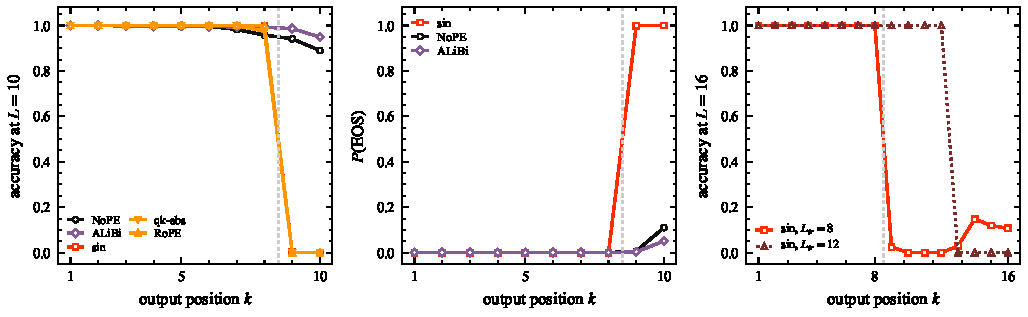
\includegraphics[width=\textwidth]{../figures/fig_profile.pdf}
\caption{The failure is a stop. (a) Accuracy at each output position, copy, test
length $10$, $L_{\mathrm{tr}}{=}8$. Sin, $q/k$-absolute and rotary are correct at
every position up to the eighth and wrong from the ninth; \nope{} and ALiBi decay
gently. The vertical line marks $L_{\mathrm{tr}}$. (b) Probability assigned to EOS
at the same positions: $1.00$ from the ninth for sin, below $0.1$ throughout for
\nope{} and ALiBi. (c) The boundary follows the training length: with
$L_{\mathrm{tr}}{=}12$ the same code is correct to the twelfth position at
$L{=}16$, and at $L{=}8$ it truncates at the eighth. Means over two seeds except
(c)'s $L_{\mathrm{tr}}{=}12$ run, which is a single run.}
\label{fig:profile}
\end{figure}


\paragraph{What we find.} On a copy task, at $L_{\mathrm{tr}}{=}8$:

\begin{itemize}[leftmargin=1.1em,itemsep=1pt,topsep=2pt]
\item \textbf{The failure is a stop.} With sin, rotary, or learned position, the
  model is correct at every output position up to the eighth and wrong at every
  position after it, for every test length; its EOS probability is $1.00$ at the
  ninth. Forced to produce ten tokens, it scores $0.93$ (sin) and $1.00$ (rotary)
  token accuracy where exact match is $0.00$ (\secref{sec:stop}).
\item \textbf{Position ranges are irrelevant.} Fixing the total token count at 41
  and padding the tail means all 41 positions occur in every training example. The
  collapse is unchanged (\secref{sec:padded}).
\item \textbf{Neither the site nor absoluteness explains it.} An absolute code
  injected at $q/k$ truncates exactly like one added to the residual stream, and
  rotary---relative by construction---truncates too. What separates the codes is
  whether the model can address the answer boundary (\secref{sec:which}).
\item \textbf{Remove the boundary and the ranking reverses.} Trained without any EOS
  token, rotary copy is perfect at $L{=}16$ ($1.00$ exact match, two seeds) while
  \nope{} falls to $0.43$ token accuracy (\secref{sec:noeos}). The code that
  ``cannot extrapolate'' extrapolates furthest once it is not asked to stop.
\end{itemize}

\paragraph{What follows.} The practical consequence is a measurement one: a PE
comparison by exact match measures termination policy as much as computation, and
reporting forced-length accuracy beside it costs nothing at evaluation time. The
scientific consequence is narrower than it looks---we study copying, small models
and two seeds---but it is directional: the diagnosis ``explicit codes put the model
out of distribution'' is not what the data show. What the data show is that an
addressable boundary gets used.

\section{Related Work}
\label{sec:related}

\paragraph{Length generalisation and positional encodings.} Transformers fit short
sequences and degrade sharply beyond them
\citep{anil2022exploring,deletang2023neural}. The explanations offered are mostly
computational: attention of fixed depth cannot represent certain length-dependent
functions \citep{hahn2020theoretical}; a task extrapolates when it admits a short
program over attention primitives \citep{weiss2021thinking,zhou2023what}; shallow
models learn shortcuts that fit the training lengths and break outside them
\citep{liu2023shortcuts}. Orthogonal to this is the choice of positional code---a
distinct vector per position \citep{vaswani2017attention}, or pairwise information
injected through learned relative representations \citep{shaw2018self}, bucketed
biases \citep{raffel2020exploring}, rotations \citep{su2024roformer} or a linear
distance penalty \citep{press2022train}---together with a family of schemes built for
the extrapolation regime: log-decaying biases \citep{chi2023dissecting},
resolution-maximising codes \citep{sun2023length}, randomised position sampling
\citep{ruoss2023randomized}, and priming with long examples
\citep{jelassi2023length}; \citet{zhao2024survey} survey the family. The headline
result is that no positional encoding beats five explicit alternatives across ten
tasks \citep{kazemnejad2023impact}, with follow-up work bounding how far that holds
and tracing the residual breakdown to unfocused attention \citep{wang2024length}.
Almost all of it is scored by exact match.

\paragraph{The EOS decision.} A separate literature studies the decision to predict an
end-of-sequence token at all. \citet{newman2020eos} show that models trained to predict
EOS extrapolate substantially worse than models that are not, trace the difference to
hidden states that stratify by position and then stall, and evaluate in the
oracle-length setting we adopt in \secref{sec:stop}. Their experiments vary the EOS
decision and hold the architecture fixed; ours varies the positional encoding and holds
the EOS decision fixed, then removes it---which is what connects the two literatures.
Small algorithmic models are the usual place to look for mechanism---grokking as a
transition from memorisation to a structured circuit
\citep{power2022grokking,nanda2023progress}, induction heads as a copying mechanism
\citep{olsson2022induction}---and we offer behaviour of that kind rather than a circuit
analysis: the profile in \figref{fig:profile} constrains what such an account must
explain, but does not localise the computation.

\section{Where Position Can Enter, and What a Boundary Is}
\label{sec:method}

Every encoding we compare is a special case of a single causal attention layer,
\begin{equation}
\mathrm{Attn}(Q,K,V)_i
= \sum_{j\le i}
\frac{\exp\!\left(\langle q_i,k_j\rangle/\sqrt{d_h} + B_{ij}\right)}
{\sum_{j'\le i}\exp\!\left(\langle q_i,k_{j'}\rangle/\sqrt{d_h} + B_{ij'}\right)}\,
v_j ,
\label{eq:attn}
\end{equation}
with $q_i=W_Q h_i$, $k_j=W_K h_j$, $v_j=W_V h_j$ and $h_i$ the residual stream at
position $i$. Position can enter at exactly three sites:
\begin{enumerate}[leftmargin=1.4em,itemsep=0pt,topsep=1pt]
\item[(i)] the token representation, $h_i = e(x_i) + p_i$, with $p_i$ learned or a
  fixed sinusoid (learned, sin);
\item[(ii)] the query/key geometry, $q_i \mapsto R_{\Theta,i}q_i$ or
  $q_i \mapsto q_i + W_q p_i$ (rotary, $q/k$-absolute);
\item[(iii)] the logits, through a bias $B_{ij}$ that carries no token content
  (ALiBi);
\end{enumerate}
and \nope{} is the fourth case, in which all three are left untouched and order is
conveyed only by the causal mask $j\le i$.

\paragraph{The logits site cannot host an absolute code.} This removes one cell from
the design and explains a gap in the literature. Suppose a bias decomposes as
$B_{ij} = c_i + B'_{ij}$, with a component that depends on the query index alone.
For fixed $i$, $c_i$ appears in every term of both the numerator and the denominator
of \eqref{eq:attn} and cancels:
\begin{equation}
\frac{e^{c_i}e^{s_{ij}}}{\sum_{j'} e^{c_i}e^{s_{ij'}}}
= \frac{e^{s_{ij}}}{\sum_{j'} e^{s_{ij'}}}, \qquad s_{ij}=\langle q_i,k_j\rangle/\sqrt{d_h}.
\label{eq:shift}
\end{equation}
An additive position signal that is constant along the key axis is therefore
unobservable. Any logits code that has an effect must vary with $j$ as well as $i$;
it is a function of the \emph{pair}. This is why every effective logits code in the
literature---ALiBi, T5 buckets, relative bias generally---is relative, and why
``absolute at the logits'' is not a condition one can run. It also means the usual
battery confounds site with kind: all absolute codes sit at site (i), and the only
codes at sites (ii) and (iii) are relative. The $q/k$-absolute condition of
\eqref{eq:qkabs} exists to break that confound.

\paragraph{Boundaries.} Write $y_1\ldots y_L$ for the answer segment and
$\mathrm{stop}(x)$ for the index at which a trained model emits EOS when run
autoregressively. We say the model \emph{truncates} when $\mathrm{stop}(x) < L$: it
produces a prefix and then declines to continue, rather than producing $L$ tokens of
which some are wrong. These are different failures and exact match reports them
identically.

A code is \emph{addressable} if, at generation time, the model can compute a quantity
that selects a particular output index independently of the token content at that
index---an absolute index, or an absolute rotation applied at a known index. \nope{}
cannot: the only positional information is the causal mask, which orders positions
without labelling them. ALiBi cannot: its bias is a function of $i-j$, which orders
output positions by distance without naming any of them. The distinction is not
absolute-versus-relative---rotary is relative and addressable---and not which site
the code occupies, since \eqref{eq:qkabs} shows an absolute code at site (ii)
behaving like one at site (i). It is about what the model can refer to, and
\secref{sec:which} tests whether it predicts which codes truncate.

\section{Experimental Setup}
\label{sec:setup}

\paragraph{Tasks.} All five tasks map a sequence of $L$ symbols from a
10-symbol alphabet to an output sequence of the same length, formatted as
\texttt{x\textsubscript{1..L} <SEP> y\textsubscript{1..L} <EOS>}. Cross-entropy
is applied only to the output segment. Training uses $L_{\mathrm{tr}}=8$; unless
stated otherwise evaluation uses $L\in\{8,10,12,16,20\}$, so $L{=}8$ measures
in-distribution fit and the rest measure extrapolation.

\paragraph{Two protocols.} Under the \emph{standard} protocol the sequence has
length $2L+2$, so the absolute position of \texttt{<SEP>} is $L$ and the answer
occupies positions $L{+}1$ to $2L$. ``The model runs out of trained positions''
and ``the model runs out of trained lengths'' are then the same event, which makes
the standard protocol unable to distinguish the account we test from the one we
reject. Under the \emph{fixed-length} protocol we hold the total token count at
$T{=}41$, pin \texttt{<SEP>} at index $K{=}21$, and fill both sides with padding:
\begin{equation}
\underbrace{x_1\ldots x_L}_{\text{input}}\;
\underbrace{\varnothing^{K-L}}_{\text{pad}}\;
\texttt{<SEP>}\;
\underbrace{y_1\ldots y_L}_{\text{answer}}\;
\texttt{<EOS>}\;
\underbrace{\varnothing^{T-K-L-2}}_{\text{pad}},
\label{eq:fixed}
\end{equation}
with $T\gg L_{\max}$. Every one of the 41 positions therefore occurs in every
training example; only the number of \emph{effective} tokens varies. If the
collapse survives this---if it appears at $L_{\mathrm{tr}}{+}2$ when no position is
new---then it cannot be an out-of-distribution position effect.

\paragraph{Positional encodings.} All conditions are instantiations of
\eqref{eq:attn}. \nope{} sets $p_i=0$, $B_{ij}=0$ and applies no rotation, so
order is conveyed only by the causal mask. \emph{learned} absolute embeddings use
$h_i=e(x_i)+p_i$ with $p_i\in\mathbb{R}^{d}$ trained, one vector per position.
\emph{sin} uses the fixed sinusoid of \citet{vaswani2017attention},
\begin{equation}
p_{i,2k}=\sin\!\left(i\,\omega_k\right),\qquad
p_{i,2k+1}=\cos\!\left(i\,\omega_k\right),\qquad
\omega_k=10000^{-2k/d}.
\label{eq:sin}
\end{equation}
\emph{rope} rotates queries and keys within each head,
$q_i\mapsto R_{\Theta,i}\,q_i$ with $R_{\Theta,i}$ block-diagonal in
$2\times2$ rotations of angle $i\theta_k$ and $\theta_k=10000^{-2k/d}$, so that
$\langle q_i,k_j\rangle$ depends on $i-j$ alone \citep{su2024roformer}.
\emph{alibi} leaves the residual stream untouched and sets
\begin{equation}
B_{ij}=-m_h\,(i-j),\qquad m_h=2^{-8h/H},
\label{eq:alibi}
\end{equation}
for head $h\in\{1,\dots,H\}$ \citep{press2022train}. Finally \emph{qk-abs} adds the
\emph{same} fixed sinusoid of \eqref{eq:sin}, linearly projected, to queries and
keys rather than to the residual stream:
\begin{equation}
q_i \leftarrow q_i + W_q p_i,\qquad k_j \leftarrow k_j + W_k p_j .
\label{eq:qkabs}
\end{equation}
This condition exists to separate two variables that the usual battery confounds:
every absolute code in the literature enters at the representation, and the only
codes at $q/k$ or at the logits are relative ones. \emph{qk-abs} is an absolute
code at a pairwise site, so a difference between it and \emph{sin} is a site
effect, and a difference between it and \emph{rope} is an absoluteness effect.
Four of the five original conditions---\nope{}, learned absolute, rotary and
ALiBi---appear in the comparison of \citet{kazemnejad2023impact}. We substitute a
fixed sinusoidal code for their T5-style bucketed relative bias
\citep{raffel2020exploring}, so our battery overlaps with theirs rather than
reproducing it; we record the substitution explicitly because it limits how
directly the numbers can be compared across the two studies.

\paragraph{Model and optimisation.} A decoder-only Transformer with 4 layers,
$d_{\mathrm{model}}{=}256$, 8 heads, pre-layered-norm blocks, GELU MLP with hidden
width $4d$, and a tied output head: about 3.2M parameters. AdamW with learning rate
$5\times10^{-4}$, $\beta=(0.9,0.98)$, weight decay $0.01$, batch size 128, 2000
steps, 100-step linear warmup then cosine decay, gradients clipped to norm 1.0.
Each step draws a fresh batch rather than sampling a fixed finite training set, so
every condition sees the same number of i.i.d.\ examples and memorisation of a
particular sample cannot explain a difference.

\paragraph{Four measurements.} Exact match is a conjunction over $L$ tokens, so it
reports a stop and a computation as the same zero. We therefore report, for each
condition and length,
\begin{enumerate}[leftmargin=1.4em,itemsep=0pt,topsep=1pt]
\item $\mathrm{Acc}_L$: sequence exact match, the standard metric;
\item $\mathrm{Tok}_L$: per-token accuracy over the answer segment, which separates
  a wrong token from a missing one;
\item $\mathrm{Acc}^{\mathrm{ora}}_L$: exact match with the EOS logit masked at
  every answer position, so generation cannot terminate early and the model is
  forced to produce $L$ tokens. This is the oracle-length evaluation used by
  \citet{newman2020eos}, and it measures content alone;
\item $\mathrm{stop}_L$: the mean index of the first position predicted as EOS,
  with $L$ recorded when no EOS is predicted.
\end{enumerate}
A model that stops at $\mathrm{stop}_L = L_{\mathrm{tr}} < L$ truncates; a model
with $\mathrm{stop}_L \approx L$ terminates correctly and fails, if at all, on
content.

\paragraph{The solved control.} A condition counts as \emph{solved} if
in-distribution accuracy at $L{=}8$ reaches $0.95$. Extrapolation failure is only
interpretable for models that learned the task; without this control a code can
appear to ``fail to extrapolate'' when it failed to fit. Unsolved conditions are
reported rather than dropped.

\paragraph{Seeds and standard errors.} Each cell is run with 2 seeds and every
figure reports the mean with the seed spread; every quoted number is the mean over
seeds. With two seeds the design is underpowered for fine pairwise claims, so we
restrict ourselves to differences that are an order of magnitude apart---which,
as \secref{sec:results} shows, is the scale of the effects here: the quantities we
contrast are $0.00$ against $0.91$ and $8$ against $10$, not $0.41$ against
$0.44$.

\section{Results}
\label{sec:results}

All 25 cells are solved by our criterion (in-distribution accuracy $\ge 0.95$;
the minimum observed is $0.998$), so every comparison below is between models
that learned the task.

\begin{table}[t]
\centering
\small
\caption{Extrapolation score ES (mean exact-match accuracy over $L\in\{10,12,16,20\}$),
averaged over seeds and restricted to solved runs. Best per row in bold. Two
length-coupled tasks are marked $^{\dagger}$. Every cell using an explicit
additive or rotary code sits at $0.00$; only ALiBi on copy departs from the
pattern.}
\label{tab:main}
\begin{tabular}{@{}lccccc@{}}
\toprule
Task & \nope{} & learned & sin & RoPE & ALiBi \\
\midrule
copy                    & \textbf{0.34} & 0.00 & 0.00 & 0.00 & 0.31 \\
prefix-XOR              & \textbf{0.00} & 0.00 & 0.00 & 0.00 & 0.00 \\
sort                    & \textbf{0.76} & 0.00 & 0.00 & 0.00 & 0.00 \\
swap-halves$^{\dagger}$ & 0.00 & 0.00 & 0.00 & 0.00 & 0.00 \\
reverse$^{\dagger}$     & \textbf{0.29} & 0.00 & 0.00 & 0.00 & 0.00 \\
\bottomrule
\end{tabular}
\end{table}

\paragraph{The cliff is not specific to one task.} \figref{fig:curves} repeats the
pattern of \figref{fig:padded} across the battery. With a learned, sinusoidal or
rotary code, accuracy is $1.00$ at the training length and $0.00$ at the next one
tested, on every task where the task can be learned at all. \nope{} instead decays
smoothly where the task permits extrapolation (copy $0.96$ at $L{=}10$, reverse
$0.87$, sort $1.00$). Twenty-one of the twenty-five cells have ES below $0.01$,
eighteen exactly zero; the discrimination between methods comes from the four
cells that clear it.

\paragraph{The failure is not an out-of-distribution position.} The standard
format cannot distinguish the two accounts, since $2L+1$ positions grow with $L$.
\figref{fig:padded} removes the confound: every example is padded to a fixed 41
tokens with the separator pinned at index 21, so all positions occur in training
and only the effective length varies. Under this protocol the learned and
sinusoidal codes still fall from $1.00$ at $L{=}8$ to $0.00$ at $L{=}10$, whereas
\nope{} retains $0.79$ and ALiBi $0.87$, decaying to $0.02$ and $0.10$ at
$L{=}12$. Padding costs some accuracy overall---\nope{} reaches $0.96$ at $L{=}10$
in the standard format and $0.79$ here, plausibly because half the sequence is
now filler---but the ordering is unchanged and the collapse is undiminished. With
no unseen position left to blame, the failure has to be indexed by length.

\begin{figure}[t]
\centering
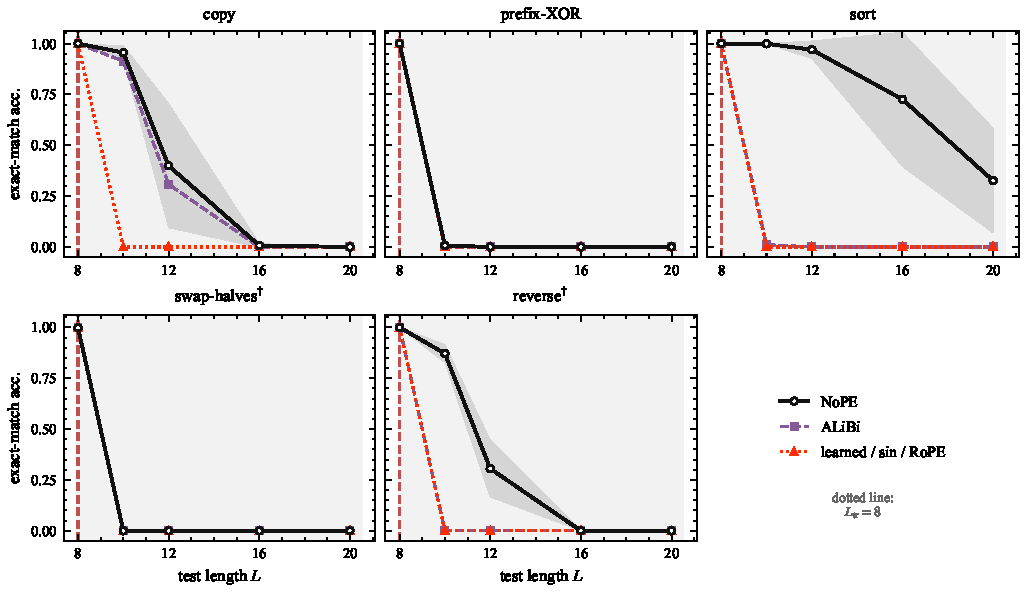
\includegraphics[width=\textwidth]{../figures/fig1_curves.pdf}
\caption{Exact-match accuracy versus test length, one panel per task, mean over
seeds with $\pm$1 s.d. The dotted line marks the training length. Learned,
sinusoidal and rotary codes coincide numerically, so they are drawn as one curve;
all three fall to zero at the first length beyond training. \nope{} instead
decays gradually on the three tasks it can extrapolate at all, and fails on the
remaining two. Tasks are ordered by length-coupling, coupled ones marked $*$.}
\label{fig:curves}
\end{figure}

\paragraph{A task-side explanation does not fit.} Before settling on the lookup
account we tested the most natural alternative: that the effect is organised by
whether a task's positional rule is written in terms of $L$ (\secref{sec:method}).
Under that account the ranking of encodings should reverse between classes, with
\nope{} losing its advantage on the coupled tasks. It does not. \nope{} is at or
near the top of every task, and the spread between the best and worst encoding is
$0.34$ (copy), $0.76$ (sort) and $0.29$ (reverse)---larger on the decoupled side
($0.37$ mean) than the coupled side ($0.15$). What the data do show is that
heterogeneity is real: a two-way ANOVA treating seed as a replicate ($n{=}50$)
gives a task$\times$encoding interaction of $F(16,25)=32.3$, $p<10^{-3}$,
$\eta_p^2=0.95$. Encodings do behave differently across tasks; the difference is
just not organised by coupling. We report this because it cuts against the
explanation we set out to test, and because a null interaction would have been a
weaker finding. The test treats seeds as independent replicates, an approximation
that if anything understates the residual variance.

\paragraph{Where every method fails, the obstacle is not positional.} On
prefix-XOR and swap-halves, \emph{every} condition including \nope{} scores at or
below $0.01$ despite reaching $\ge 0.998$ in-distribution. The obstacle there is
the difficulty of representing the underlying algorithm in a length-invariant way,
the phenomenon studied by \citet{zhou2023what}, and no choice of positional
encoding can address it. Keeping these tasks in the battery is what makes that
visible: it bounds what any PE intervention could achieve.

\section{Discussion}
\label{sec:discussion}

\paragraph{What the comparison was measuring.} The ordering in \tabref{tab:main} is
reproducible and, as a description of trained models under the usual recipe, correct.
What it does not license is the inference that explicit codes compute worse. On copy
the opposite holds: under a forced output length rotary reaches $0.996$ token
accuracy at $L{=}10$ and $0.984$ at $L{=}12$ against $0.987$ and $0.877$ for \nope{},
and with EOS removed from training rotary is perfect at $L{=}16$ while \nope{} falls
to $0.43$. The standard protocol was measuring where models stop.

\paragraph{Why the boundary lands on $L_{\mathrm{tr}}$.} A model trained at one
length sees exactly $L_{\mathrm{tr}}$ answer tokens in every example. If it can
address output positions, the rule ``emit EOS at index $L_{\mathrm{tr}}{+}1$'' is a
single parameter that fits the training distribution perfectly and is simply
undefined outside it; nothing in the objective penalises that. If it cannot address
positions, the same rule is not representable, and the model must fall back on
content or on a distance cue, both of which are fuzzier and later---which is what
the \nope{} and ALiBi profiles in \figref{fig:profile} show. The asymmetry is not
about the informativeness of the code but about whether a stop can be encoded as a
constant.

This is the mechanism behind the ``length attractor'' of \citet{newman2020eos}:
they showed that models trained to predict EOS stratify hidden states by position
and stall there, and we locate the consequence at the level of a cross-code
comparison. It is also why a mixture over lengths does not help the absolute code
(\secref{sec:moves}): the constant becomes a lookup with one entry per length, but
it is still a lookup, and the entry for the test length does not exist.

\paragraph{Relation to the no-PE recommendation.} \citet{kazemnejad2023impact}
compare five encodings on ten tasks and find \nope{} best. Our \tabref{tab:main}
reproduces that ordering on our tasks and our model size. The result here does not
overturn their measurement; it reinterprets what it measures. On tasks where the
answer has the same length as the input, an exact-match comparison is partly a
comparison of how crisply each code can place a stop. The practical corollary is
cheap: report forced-length accuracy alongside exact match, or evaluate with EOS
masked, and the comparison becomes about computation again.

\paragraph{Why ALiBi is the exception in the standard table.} ALiBi is the only
standard code that both leaves the residual stream alone and is unaddressable: its
bias orders output positions by distance from the query without naming any of them.
It therefore stops late and softly rather than at a constant, which is what its
$0.92$ exact match at $L{=}10$ reflects. We would predict that any code with a
monotone and unaddressable positional signal behaves similarly, and that ALiBi's
advantage would shrink under no-EOS training---a prediction we did not test.

\paragraph{What this does not show.} We study copying with a 3.2M-parameter model,
two seeds, and one training length per condition. \emph{sort}, \emph{reverse} and
\emph{prefix-XOR} are in \tabref{tab:main} but not in the decomposition, and the
permutation tasks may not decompose the same way, since a truncated answer there is
wrong at every position rather than at the tail. We also did not test whether the
effect survives scale, pretraining, or natural language, where answers rarely have
the same length as inputs and the boundary is cued by content rather than by a
count. The claim we are prepared to defend is the narrow one: on copy-like
same-length tasks, at this scale, the cross-code ranking on exact match is dominated
by termination, and it reverses when termination is removed.

\section{Limitations}
\label{sec:limitations}

\paragraph{Scale.} Our models have 3.2M parameters and are trained from scratch on
synthetic sequence tasks. Nothing in our argument requires scale, but nothing in
our experiments establishes that the same conditioning holds for pretrained
language models, where positional codes interact with token distributions and
with training that already spans many lengths. We regard the present study as a
controlled test of a mechanism, not as a claim about frontier models.

\paragraph{One training length.} All runs use $L_{\mathrm{tr}}{=}8$. A stronger
version of our claim would show that the coupling classification predicts the
\emph{shape} of the extrapolation curve across several training lengths, not just
the sign of a difference at one. This is the most important extension we have not
run.

\paragraph{Online sampling.} Each step draws a fresh batch rather than sampling
from a fixed finite training set. This removes memorisation as an explanation and
equalises the number of examples across conditions, but it also makes the task
easier than the fixed-train-set protocol used in some prior work, so absolute
accuracies are not directly comparable across papers.

\paragraph{Coverage of the taxonomy.} Five tasks is a small battery, and the
position-free class is represented by a single task (sort). The two coupled
tasks, while both length-dependent, differ in how the dependence enters
(complement versus rotation), so we cannot separate ``coupled'' from ``coupled in
this particular way''.

\paragraph{Confound in the learned-APE condition.} At test lengths the learned
embedding table is queried at positions never updated during training. This is
faithful to how learned absolute codes behave in deployment, but it means the
learned condition conflates ``absolute position is unhelpful'' with ``the
untrained tail of a lookup table is unhelpful''. A variant with a
length-extrapolable initialisation would separate the two; we did not run one.

\paragraph{Statistical power.} Two seeds per cell leave only 25 residual degrees
of freedom for the interaction test, and treating seeds as replicates is an
approximation. The interaction we report is far from marginal
($F(16,25)=32.3$), but the cell-level means it is computed from are noisy enough
that we would not defend a claim about any single pairwise difference. A
five-seed replication is the obvious next step and we have not run it.

\paragraph{Behavioural evidence only.} We report accuracy, not mechanism. Claims
about \emph{why} a coupled task is harder---whether models recover length from
attention statistics, whether they implement a position-arithmetic circuit---would
require probing or circuit analysis that we have not performed.

\section{Conclusion}
\label{sec:conclusion}

The question we began with was not which positional encoding is best, but what
property of a task predicts whether a positional encoding will help. We proposed
one such property---whether the task's positional rule is written in terms of the
sequence length---and tested it with a factorial design that separates ``failed to
fit'' from ``failed to extrapolate''. The answer was no: the coupling class did
not predict the sign of the effect, and \nope{} was never worse than an explicit
code, including on the two tasks constructed to favour its competitors. What we
can say with more confidence than before is narrower but firmer: the advantage of
omitting positional encoding survives the condition we designed to break it.

The broader methodological point is that recommendations about architectural
components are conditional objects. An aggregate ranking over a task battery is a
summary of a distribution, and if that distribution is heterogeneous the summary
can invert the sign of the effect for any given task. Reporting the conditioning
variable alongside the ranking costs little and makes the recommendation
actionable: a practitioner who knows their task's coupling class can choose a
positional encoding deliberately rather than by reputation.


\bibliographystyle{plainnat}
\bibliography{refs}

\end{document}
